\documentclass[12pt]{article}
\usepackage{amsmath}
\usepackage{graphicx}
\usepackage{hyperref}
\usepackage[utf8]{inputenc}
\usepackage{geometry}
\usepackage{mathtools}
\usepackage{empheq}
\usepackage{listings}
\usepackage{xcolor}
\usepackage{authblk}
\usepackage{subcaption}
\usepackage{svg}
\usepackage{minted}


\definecolor{LightGray}{gray}{0.9}

\graphicspath{ {./assets/} }
\geometry{margin=0.75in}

\title{CHEN 425}
\author{Mark L}
\date{February 2023}

\begin{document}
% \maketitle

\begin{enumerate}

% Problem 1 %%%%%%%%%%%%%%%%%%%%%%%%%%%%%%%%%%%%%%%%%%%%%%%%%%%%%%%%%%%%
\newpage
    \item Problem 3.15
    
    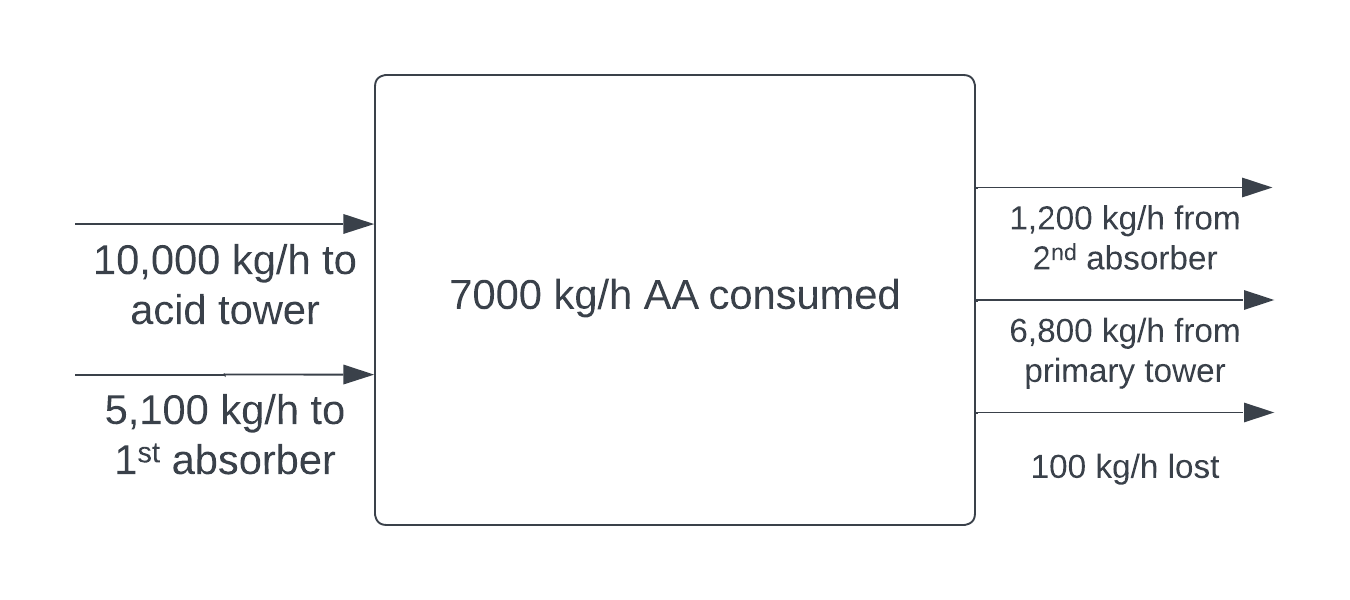
\includegraphics{assets/3.15-1.png}

    The acetic acid from the $2^{\mathrm{nd}}$ absorber and the primary column can be recovered and recylced back to the process, decreasing the necessary fresh feed by 8,000 kg/h.

    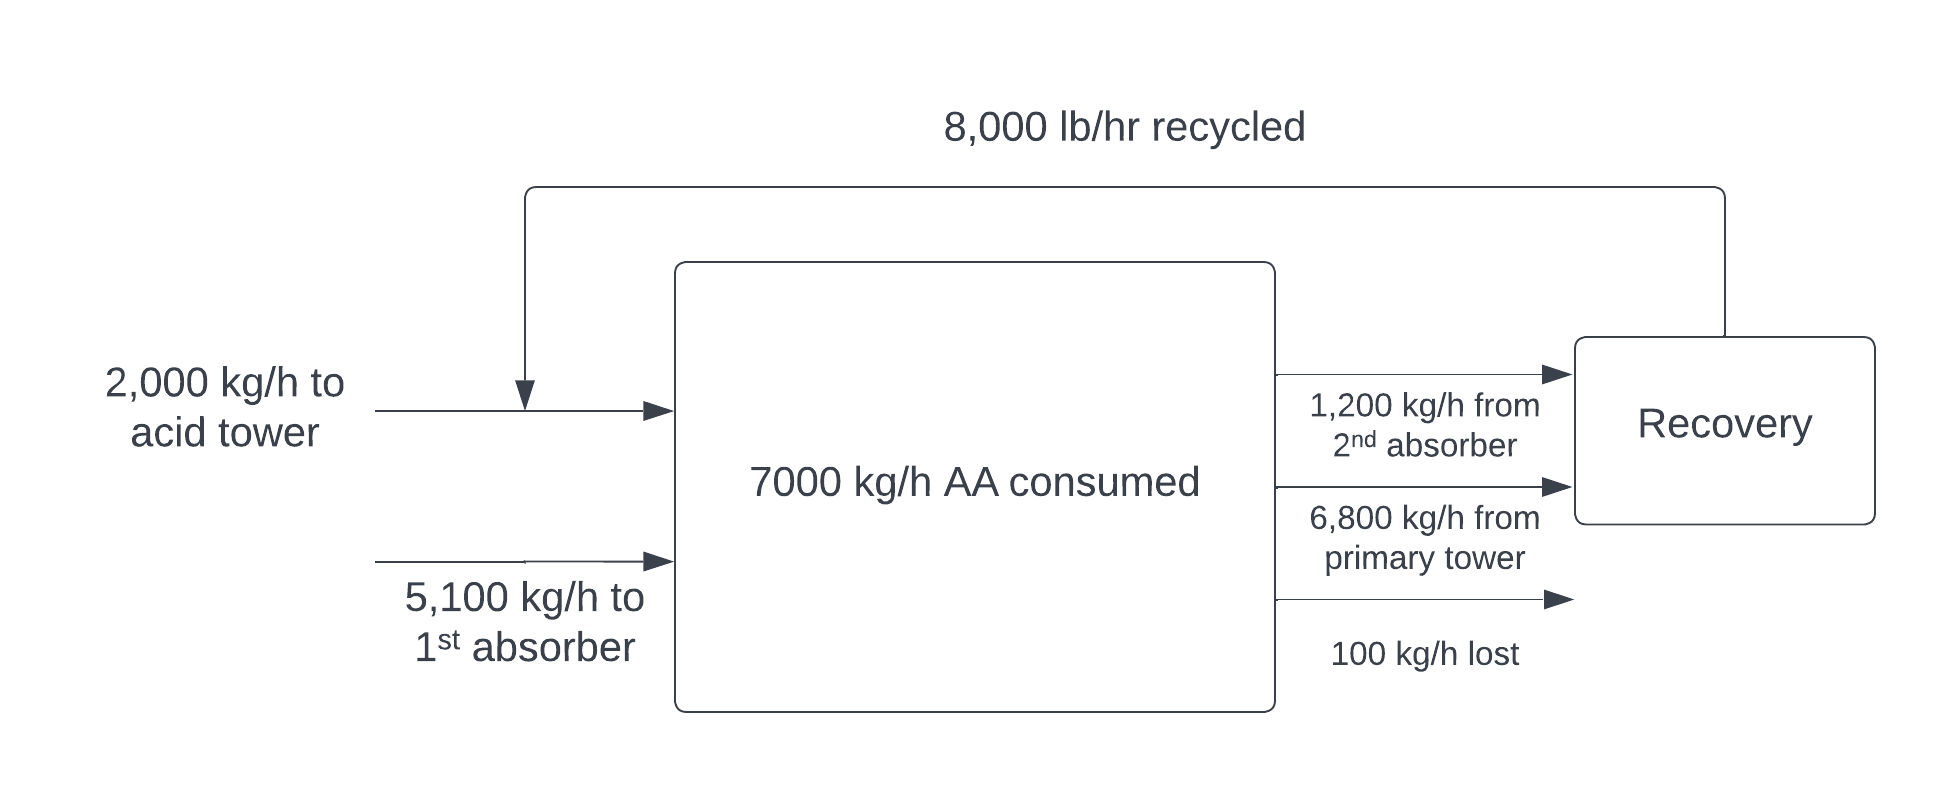
\includegraphics{assets/3.15-2.png}

    The total required fresh feed is 7,100 kg/h, and the losses are 100 kg/h.
    
% Problem 2 %%%%%%%%%%%%%%%%%%%%%%%%%%%%%%%%%%%%%%%%%%%%%%%%%%%%%%%%%%%%
\newpage
    \item Problem 3.16
    
    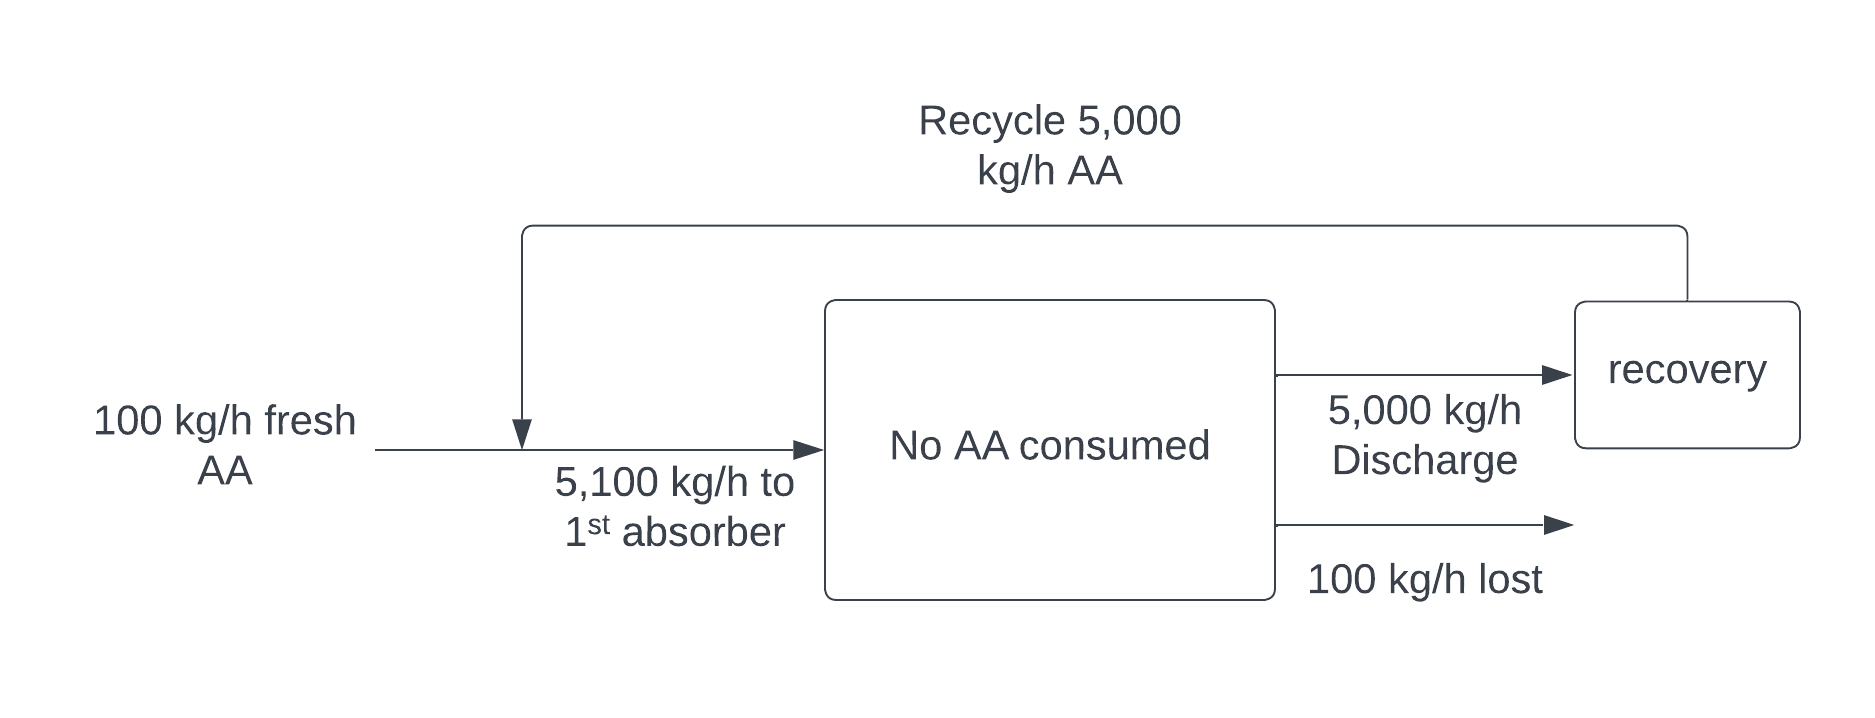
\includegraphics{assets/3.16.png}

    10,000 kg/h of acetic acid is no longer necessary to feed to the reactor. 100 kg/h is lost. The remaining 5,000 kg/h of acetic acid discharge can be recovered back to the process.

    The total required frech feed is 100 kg/h, the same as the total losses.

% Problem 3 %%%%%%%%%%%%%%%%%%%%%%%%%%%%%%%%%%%%%%%%%%%%%%%%%%%%%%%%%%%%
\newpage
    \item Problem 3.17
    
    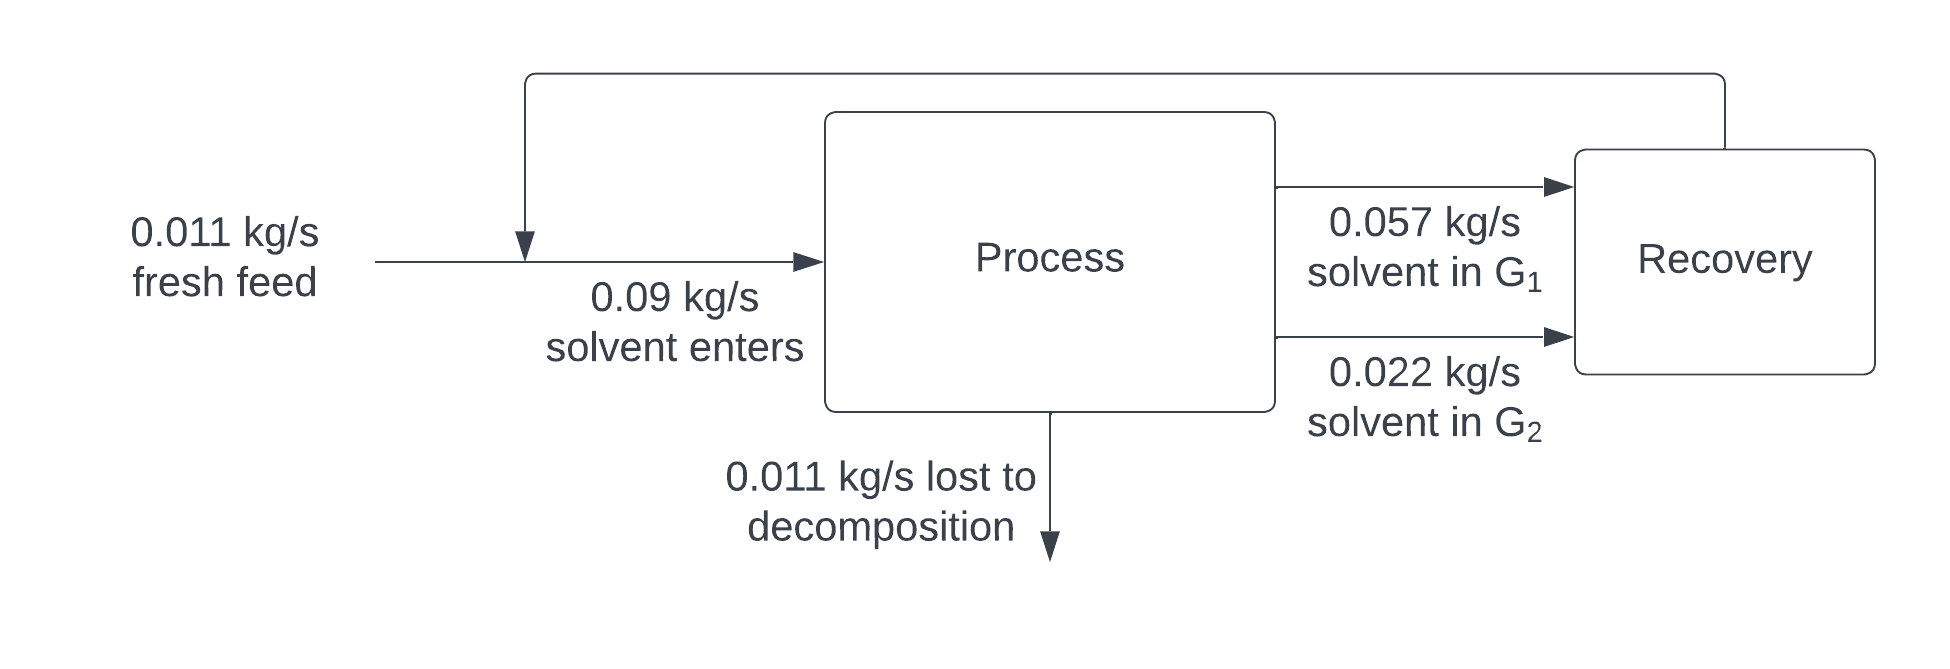
\includegraphics{assets/3.17.png}

    0.09 kg/s of solvent is fed to the process. 0.011 kg/s of solvent is lost to decomposition. 0.079 kg/s comes from G$_1$ and G$_2$. This solvent can be recovered and recycled to the feed. 

    The total required frech feed then becomes 0.011 kg/s of solvent to make up for 0.011 kg/s in losses.

% Problem 4 %%%%%%%%%%%%%%%%%%%%%%%%%%%%%%%%%%%%%%%%%%%%%%%%%%%%%%%%%%%%
\newpage
    \item Problem 3.18
    \begin{enumerate}
        \item 
        \begin{align*}
            \text{A in S1} &= 200 \\
            \text{P production} = 0.8 \cdot 200 - 2 \cdot (375 - 370)^2 &= 110 \\
            \text{Total fresh input} = 200 + 100 &= 300 \\
            \mathrm{ME} &= \frac{0.8 \cdot 110}{300} \\ 
            \Aboxed{\mathrm{ME} &= 29.3 \%}
        \end{align*}
        \item 
        \begin{align*}
            \intertext{Find the maximum of this equation:} 
            \text{P production} &= 0.8 \cdot 200 - 2 \cdot (375 - T)^2 \\  
            \Aboxed{T &= 375 \text{ K}}
        \end{align*}
        \item 
        \begin{align*}
            \intertext{From maximum solver in the last part}
            \text{P production} &= 160 \text{ kg/h} \\
            \text{P in S7} &= 160 \cdot 0.8 \\ 
            \Aboxed{\text{P in S7} &= 128 \text{ kg/h}}    
        \end{align*}
        \item 
        \begin{align*}
            \intertext{Recover all P in S2}
            \Aboxed{\text{P in S7} &= 160 \text{ kg/h}}
        \end{align*}
        \item 
        \begin{align*}
            \intertext{Recover A in S3 and B in S6}
            \text{Recovered A} &= 40 \text{ kg/h} \\
            \text{Recovered B} &= 95 \text{ kg/h} \\  
            \text{Total recovered inputs} &= 135 \text{ kg/h} \\
            \intertext{Decrease input by 135 kg/hr}
            \text{Required input} = 300 - 135 &= 165 \text{ kg/h} \\
            \text{P in S7} &= 160 \text{ kg/h} \\
            \mathrm{ME} &= \frac{160}{165} \\
            \Aboxed{\mathrm{ME} &= 97.7 \%}
        \end{align*}
    \end{enumerate}


\end{enumerate}
\end{document}
